\documentclass{parasim}
\usepackage{graphicx}
\usepackage{caption}
\usepackage{subcaption}

\title{Zpráva za období červenec až září 2012}

\begin{document}

\section{Druhá etapa}
V~druhé etapě, probíhající do konce července 2012, jsme se zabývali tvorbou testů a dokumentace,
hledáním vhodných modelů pro analýzu, profilováním a drobnými úpravami nástroje.

Během této etapy došlo k~následujícím změnám na projektu:
\begin{itemize}
	\item	byla vytvořena dokumentace k~jednotlivým rozšířením výpočtu a vizualizace,
	\item	jádro aplikace bylo refaktorováno tak, aby umožnilo vytváření dalších rozšíření,
	\item	bylo vytvořeno rozšíření pro měření výkonu aplikace,
	\item	byla vytvořena dokumentace popisující instalaci parasimu, vytvoření projektu (včetně formátu vstupních souborů) a spuštění aplikace z~příkazové řádky
	\item	aplikace spustitelná z~příkazové řádky byla doplněna o~skript zjenodušující vytvoření projektu
	\item	byly napsány testy zaměřené na některé součásti aplikace a vytvořeny testovací experimenty
\end{itemize}

Vydaná verze z~konce druhé etapy je k~dispozici na stránkách našeho projektu\footnote{\url{https://github.com/sybila/parasim/zipball/1.0.0.M2}},
kde najdete též seznam vyřešených úkolů\footnote{\url{https://github.com/sybila/parasim/issues?milestone=4&page=1&state=closed}}.

Klíčový úkol této etapy tvořilo měření výkonu jednotlivých částí aplikace. Zároveň jsme zkusili v~aplikaci analyzovat několik jednoduchých modelů z~reálného světa.

\subsection{Měření výkonu}\label{sec:performance}
Nástroj byl postupně spouštěn nad třemi dostupnými testovacími modely. Cílem bylo změřit podíl jednotlivých částí algoritmu na celkovém čase.
Konfigurace testovacího stroje byla následující:
\begin{center}
\framebox[\textwidth]{\parbox{0.9\textwidth}{\small
Java(TM) SE Runtime Environment (build 1.7.0\_04-b20), Java HotSpot(TM) 64-Bit Server VM (build 23.0-b21, mixed mode),
Linux version 2.6.43.8-1.fc15.x86\_64, Intel(R) Core(TM) i7-2620M CPU @ 2.70GHz (4 jádra), 4 GB paměti
}}
\end{center}

Obrázek \ref{fig:profiling} ukazuje na třech testovacích modelech\footnote{Testovací modely jsou součástí distribučního balíčku.},
že výrazně nejnáročnější částí výpočtu je simulace. Proto bylo rozhodnuto, že ve třetí etapě (viz \ref{sec:etapa3}) bude
věnováno úsilí jejímu zrychlení paralelizací.

\begin{figure}[h!]
	\centering
	\begin{subfigure}[b]{0.3\textwidth}
		\centering
		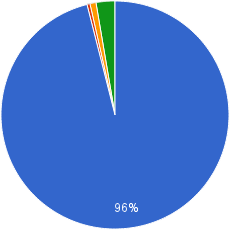
\includegraphics[width=\textwidth]{1.0.0.M2/test-1a.png}
		\caption{\texttt{test-1}}
	\end{subfigure}
	\begin{subfigure}[b]{0.3\textwidth}
		\centering
		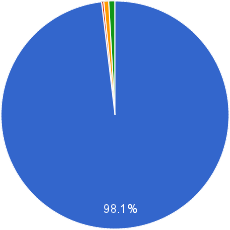
\includegraphics[width=\textwidth]{1.0.0.M2/test-2a.png}
		\caption{\texttt{test-2}}
	\end{subfigure}
	\begin{subfigure}[b]{0.3\textwidth}
		\centering
		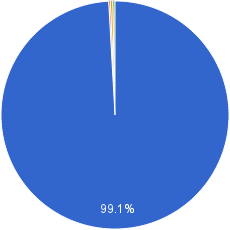
\includegraphics[width=\textwidth]{1.0.0.M2/test-3a.png}
		\caption{\texttt{test-3}}
	\end{subfigure}
	\caption{Čas strávený při jednotlivých fázích výpočtu parasimu na různých testovacích modelech.
	Modře je znázorněn čas strávený simulací, červeně zahušťováním, oranžově verifikací a zeleně vykreslením výsledku.}
	\label{fig:profiling}
\end{figure}

\subsection{Reálné modely}\label{sec:modely}
Při analýze reálných modelů vyšly najevo dvě skutečnosti:
\begin{itemize}
	\item	Většina reálných modelů, na kterých se sleduje robustnost, ji sleduje vzhledem ke změně parametrů modelů.
		Analýza robustnosti vzhledem k~parametrům však (stav na konci druhé etapy) není parasimem podporována.
	\item	Srozumitelnost výsledku analýzy je značně omezená tím, že je zobrazena pouze robustnost bez výstupů jednotlivých simulací.
\end{itemize}

Podpora pro analýzu parametrů byla zařazena mezi úkoly třetí etapy. Jelikož je srozumitelnost výsledku pro uživatele jedním
ze základních požadavků nástroje, došli jsme k~závěru, že je nutné naimplementovat grafické rozhraní, které spojuje zobrazení výsledku analýzy robustnosti
se zobrazením výsledku simulací modelu, které slouží jako podklad pro analýzu robustnosti. To však povede ke zpoždění práce na grafickém rozhraní jako celku.

\section{Třetí etapa}\label{sec:etapa3}
Ve třetí etapě, probíhající od začátku srpna do konce října, se věnujeme paralelizaci simulace a implementaci grafického rozhraní.
Práce na úkolech spojených s~touto etapou stále pokračuje, do současné doby byly provedeny následující změny:

\begin{itemize}
	\item byla přidána podpora pro analýzu parametrů (viz \ref{sec:modely})
	\item byl vytvořen framework pro paralelizaci
	% nevím, jestli tady chceš říct, že bylo paralelizováno na více jader
	\item byly naimplementovány některé komponenty grafického uživatelského rozhraní
\end{itemize}


Průběh práce na třetí etapě -- vyřešené a dosud nevyřešené úkoly -- je k~dispozici na stránkách našeho projektu\footnote{\url{https://github.com/sybila/parasim/issues?milestone=2&page=1}}.

\end{document}
